% ═══════════════════════════════════════════════════════════════════════════
%  DDF — préambule commun aux sept articles.  % ═══════════════════════════════════════════════════════════════════════════
%  DDF — préambule commun aux sept articles.  % ═══════════════════════════════════════════════════════════════════════════
%  DDF — préambule commun aux sept articles.  \input{ddf-common} en tête.
%  Définit : la mise en page, les macros, le bloc de série, la déclaration
%  d'usage d'outils, et le bloc de traçabilité.
% ═══════════════════════════════════════════════════════════════════════════
\documentclass[11pt,a4paper]{article}
\usepackage[margin=2.3cm]{geometry}
\usepackage{amsmath,amssymb,booktabs,hyperref,graphicx,xcolor}
\usepackage[expansion=false]{microtype}
\hypersetup{colorlinks=true,linkcolor=blue!45!black,citecolor=blue!45!black,urlcolor=blue!45!black}

% ---------- macros physiques ----------
\newcommand{\MPl}{M_{\rm Pl}}\newcommand{\Mred}{\bar M_{\rm Pl}}
\newcommand{\Mfive}{M_5}\newcommand{\MS}{M_S}\newcommand{\V}{\mathcal V}
\newcommand{\Neff}{N_{\rm eff}}\newcommand{\cb}{c_b}\newcommand{\ab}{\alpha_b}

% ---------- étiquettes épistémiques ----------
\newcommand{\Derived}{\textit{[Derived]}}
\newcommand{\Input}{\textit{[Input, natural]}}
\newcommand{\Posited}{\textit{[Posited]}}
\newcommand{\Candidate}{\textit{[Candidate]}}
\newcommand{\Open}{\textit{[Open, declared]}}
\newcommand{\Verified}{\textit{[Verified]}}

% ---------- bloc de série : \seriesdate{III}{The medium} ----------
\newcommand{\seriesdate}[2]{%
 \date{\small \textit{Cosmic Shadow Geometry} \\ \small Article #1 of VII
 \,\textperiodcentered\, #2 \,\textperiodcentered\, \today}}

% ---------- déclaration d'outils, identique dans les sept ----------
\newcommand{\toolsstatement}{%
\section*{Declaration on computational tools}
\addcontentsline{toc}{section}{Declaration on computational tools}
\small
This work was carried out by the author alone, without institutional affiliation.
\textbf{Large language models were used as computational and analytical assistants
throughout}: to write and debug the numerical scripts, to run the scans and
minimisations, to produce the figures, to check algebra and dimensional
consistency, to search and summarise the literature, and to audit drafts for
internal contradictions. Several distinct systems were used and cross-checked
against one another; no single system's output was accepted without an
independent numerical or analytical verification.

\textbf{The author is solely responsible for the physical hypotheses, the
interpretation of every result, the epistemic labels attached to each claim, and
the decision of what to publish and what to withdraw.} All quantitative
statements in this paper are reproduced by the scripts listed in the
traceability section; a reader who runs them obtains the numbers printed here
without needing any language model. Where an earlier draft contained an error
introduced by an unverified computation, it is recorded as a withdrawal rather
than silently removed.
\normalsize}

% ---------- bloc de traçabilité : \traceability{V}{...} ----------
\newcommand{\traceability}[2]{%
\section*{Data availability, traceability and reproducibility}
\addcontentsline{toc}{section}{Traceability}
\small
Every number, table and figure in this paper is regenerated by the scripts of
this article's folder. The complete repository ---sources, scripts, proof files,
figures and compiled documents for all seven articles--- is at
\url{https://github.com/HBoufourou}.

\textbf{Folder \texttt{article-#1/} contains:}
\begin{itemize}\itemsep2pt
\item \texttt{tex/} --- the \LaTeX\ source and the shared preamble \texttt{ddf-common.tex};
\item \texttt{scripts/} --- every computation, each runnable standalone with
      \texttt{python3 <name>.py} and printing its own verification verdict;
\item \texttt{proofs/} --- the JSON files carrying the certified values.
      \textbf{Any number absent from \texttt{proofs/} is not certified};
\item \texttt{data/} --- the CSV tables underlying the figures;
\item \texttt{figures/} --- the PNG files, regenerated by \texttt{scripts/figures.py};
\item \texttt{pdf/} --- the compiled article;
\item \texttt{VERIFICATION.txt} --- the output of the verification suite.
\end{itemize}
#2
\normalsize}
 en tête.
%  Définit : la mise en page, les macros, le bloc de série, la déclaration
%  d'usage d'outils, et le bloc de traçabilité.
% ═══════════════════════════════════════════════════════════════════════════
\documentclass[11pt,a4paper]{article}
\usepackage[margin=2.3cm]{geometry}
\usepackage{amsmath,amssymb,booktabs,hyperref,graphicx,xcolor}
\usepackage[expansion=false]{microtype}
\hypersetup{colorlinks=true,linkcolor=blue!45!black,citecolor=blue!45!black,urlcolor=blue!45!black}

% ---------- macros physiques ----------
\newcommand{\MPl}{M_{\rm Pl}}\newcommand{\Mred}{\bar M_{\rm Pl}}
\newcommand{\Mfive}{M_5}\newcommand{\MS}{M_S}\newcommand{\V}{\mathcal V}
\newcommand{\Neff}{N_{\rm eff}}\newcommand{\cb}{c_b}\newcommand{\ab}{\alpha_b}

% ---------- étiquettes épistémiques ----------
\newcommand{\Derived}{\textit{[Derived]}}
\newcommand{\Input}{\textit{[Input, natural]}}
\newcommand{\Posited}{\textit{[Posited]}}
\newcommand{\Candidate}{\textit{[Candidate]}}
\newcommand{\Open}{\textit{[Open, declared]}}
\newcommand{\Verified}{\textit{[Verified]}}

% ---------- bloc de série : \seriesdate{III}{The medium} ----------
\newcommand{\seriesdate}[2]{%
 \date{\small \textit{Cosmic Shadow Geometry} \\ \small Article #1 of VII
 \,\textperiodcentered\, #2 \,\textperiodcentered\, \today}}

% ---------- déclaration d'outils, identique dans les sept ----------
\newcommand{\toolsstatement}{%
\section*{Declaration on computational tools}
\addcontentsline{toc}{section}{Declaration on computational tools}
\small
This work was carried out by the author alone, without institutional affiliation.
\textbf{Large language models were used as computational and analytical assistants
throughout}: to write and debug the numerical scripts, to run the scans and
minimisations, to produce the figures, to check algebra and dimensional
consistency, to search and summarise the literature, and to audit drafts for
internal contradictions. Several distinct systems were used and cross-checked
against one another; no single system's output was accepted without an
independent numerical or analytical verification.

\textbf{The author is solely responsible for the physical hypotheses, the
interpretation of every result, the epistemic labels attached to each claim, and
the decision of what to publish and what to withdraw.} All quantitative
statements in this paper are reproduced by the scripts listed in the
traceability section; a reader who runs them obtains the numbers printed here
without needing any language model. Where an earlier draft contained an error
introduced by an unverified computation, it is recorded as a withdrawal rather
than silently removed.
\normalsize}

% ---------- bloc de traçabilité : \traceability{V}{...} ----------
\newcommand{\traceability}[2]{%
\section*{Data availability, traceability and reproducibility}
\addcontentsline{toc}{section}{Traceability}
\small
Every number, table and figure in this paper is regenerated by the scripts of
this article's folder. The complete repository ---sources, scripts, proof files,
figures and compiled documents for all seven articles--- is at
\url{https://github.com/HBoufourou}.

\textbf{Folder \texttt{article-#1/} contains:}
\begin{itemize}\itemsep2pt
\item \texttt{tex/} --- the \LaTeX\ source and the shared preamble \texttt{ddf-common.tex};
\item \texttt{scripts/} --- every computation, each runnable standalone with
      \texttt{python3 <name>.py} and printing its own verification verdict;
\item \texttt{proofs/} --- the JSON files carrying the certified values.
      \textbf{Any number absent from \texttt{proofs/} is not certified};
\item \texttt{data/} --- the CSV tables underlying the figures;
\item \texttt{figures/} --- the PNG files, regenerated by \texttt{scripts/figures.py};
\item \texttt{pdf/} --- the compiled article;
\item \texttt{VERIFICATION.txt} --- the output of the verification suite.
\end{itemize}
#2
\normalsize}
 en tête.
%  Définit : la mise en page, les macros, le bloc de série, la déclaration
%  d'usage d'outils, et le bloc de traçabilité.
% ═══════════════════════════════════════════════════════════════════════════
\documentclass[11pt,a4paper]{article}
\usepackage[margin=2.3cm]{geometry}
\usepackage{amsmath,amssymb,booktabs,hyperref,graphicx,xcolor}
\usepackage[expansion=false]{microtype}
\hypersetup{colorlinks=true,linkcolor=blue!45!black,citecolor=blue!45!black,urlcolor=blue!45!black}

% ---------- macros physiques ----------
\newcommand{\MPl}{M_{\rm Pl}}\newcommand{\Mred}{\bar M_{\rm Pl}}
\newcommand{\Mfive}{M_5}\newcommand{\MS}{M_S}\newcommand{\V}{\mathcal V}
\newcommand{\Neff}{N_{\rm eff}}\newcommand{\cb}{c_b}\newcommand{\ab}{\alpha_b}

% ---------- étiquettes épistémiques ----------
\newcommand{\Derived}{\textit{[Derived]}}
\newcommand{\Input}{\textit{[Input, natural]}}
\newcommand{\Posited}{\textit{[Posited]}}
\newcommand{\Candidate}{\textit{[Candidate]}}
\newcommand{\Open}{\textit{[Open, declared]}}
\newcommand{\Verified}{\textit{[Verified]}}

% ---------- bloc de série : \seriesdate{III}{The medium} ----------
\newcommand{\seriesdate}[2]{%
 \date{\small \textit{Cosmic Shadow Geometry} \\ \small Article #1 of VII
 \,\textperiodcentered\, #2 \,\textperiodcentered\, \today}}

% ---------- déclaration d'outils, identique dans les sept ----------
\newcommand{\toolsstatement}{%
\section*{Declaration on computational tools}
\addcontentsline{toc}{section}{Declaration on computational tools}
\small
This work was carried out by the author alone, without institutional affiliation.
\textbf{Large language models were used as computational and analytical assistants
throughout}: to write and debug the numerical scripts, to run the scans and
minimisations, to produce the figures, to check algebra and dimensional
consistency, to search and summarise the literature, and to audit drafts for
internal contradictions. Several distinct systems were used and cross-checked
against one another; no single system's output was accepted without an
independent numerical or analytical verification.

\textbf{The author is solely responsible for the physical hypotheses, the
interpretation of every result, the epistemic labels attached to each claim, and
the decision of what to publish and what to withdraw.} All quantitative
statements in this paper are reproduced by the scripts listed in the
traceability section; a reader who runs them obtains the numbers printed here
without needing any language model. Where an earlier draft contained an error
introduced by an unverified computation, it is recorded as a withdrawal rather
than silently removed.
\normalsize}

% ---------- bloc de traçabilité : \traceability{V}{...} ----------
\newcommand{\traceability}[2]{%
\section*{Data availability, traceability and reproducibility}
\addcontentsline{toc}{section}{Traceability}
\small
Every number, table and figure in this paper is regenerated by the scripts of
this article's folder. The complete repository ---sources, scripts, proof files,
figures and compiled documents for all seven articles--- is at
\url{https://github.com/HBoufourou}.

\textbf{Folder \texttt{article-#1/} contains:}
\begin{itemize}\itemsep2pt
\item \texttt{tex/} --- the \LaTeX\ source and the shared preamble \texttt{ddf-common.tex};
\item \texttt{scripts/} --- every computation, each runnable standalone with
      \texttt{python3 <name>.py} and printing its own verification verdict;
\item \texttt{proofs/} --- the JSON files carrying the certified values.
      \textbf{Any number absent from \texttt{proofs/} is not certified};
\item \texttt{data/} --- the CSV tables underlying the figures;
\item \texttt{figures/} --- the PNG files, regenerated by \texttt{scripts/figures.py};
\item \texttt{pdf/} --- the compiled article;
\item \texttt{VERIFICATION.txt} --- the output of the verification suite.
\end{itemize}
#2
\normalsize}

\graphicspath{{figures/}{../figures/}}
\title{\textbf{The Dark Dimension Framework VI:\\ What the candidate geometry implies ---\\ one wall, geometric dark energy, and fibre inflation}}
\author{Hicham Boufourou\\ \small\textit{Independent Researcher, Brussels, Belgium}\\ \small\texttt{hicham.boufourou@hotmail.com}}
\seriesdate{VI}{What the candidate geometry implies}
\begin{document}\maketitle
\begin{abstract}
\noindent Article~V identifies an explicit Type~I$'$ vacuum --- polytope 3181 of the orientifold database, $h^{1,1}=5$, $h^{2,1}=81$, $\chi=-152$ --- and shows that its K3 wrapping reaches the phenomenological window. This companion asks what \emph{else} that geometry implies, in two parts. \textbf{Part~A} reads the D8 brane as a single wall carrying seven regions and derives three things: an exact sum rule $\alpha_b^2+\alpha_b'^2=2w_1|\vec p|^2=2.2414$ that protects the fifth-force observable from the incalculable loop coefficients; a topological wall that pins $R$ to $8.34\,\mu$m against the framework's $8.2\,\mu$m; and a geometric reading of dark energy as extrinsic curvature, $\Lambda_4=\varepsilon^2(1/R)^4$ with $\varepsilon\simeq10^{-2}$, which replaces a forty-order engine gap by a four-order one. A predictive layer follows --- $\Omega_{\rm DM}/\Omega_b=N_{\rm regions}-1=6$ against $5.31$ --- with its fitted factor declared. \textbf{Part~B} runs fibre inflation on the same vacuum: the candidate carries exactly one K3 divisor, fixed by the orientifold involution and hence even, so the inflaton is forced rather than chosen; the observables depend on $N_e$ alone, $n_s\simeq0.969$, $r\simeq0.005$, $r\simeq6(n_s-1)^2$; and the Planck amplitude fixes $M_{\rm inf}\simeq6.7\times10^{15}$~GeV by a chain that contains no intersection number. \textbf{Two withdrawals are recorded.} A radion/Cassini mechanism from an earlier draft is removed: the tension it resolved does not exist, and its warp factor contradicts the linear well of Article~II. And an earlier anchoring of the inflation calculation on a manifold with $h^{2,1}=121$ is corrected; the physical result survives, its geometric justification did not.
\end{abstract}

\section{One geometry, two questions}
The parent series~\cite{DDF1,DDF2,DDF3,DDF4} fixes an $8.2\,\mu$m interval, a dark scalar of mass $24$~meV, and a Standard Model on a thin core at one boundary. Article~V embeds the boundary conditions in Type~I$'$ and finds one geometry, among an enumerated family of about twenty, whose K3 wrapping reaches the coupling window. This paper takes that geometry as given and asks two questions the coupling calculation did not: what does the \emph{wall} do, and what does the \emph{fibre} do. The two questions share every input --- the same divisor content, the same involution, the same intersection numbers --- and are treated together for that reason.

\begin{figure}[h]\centering
\includegraphics[width=.92\textwidth]{fig_divisors_3181}
\caption{The nine toric divisors of polytope 3181 with their types, and the orientifold involution read from the database. Three pairs are exchanged --- both dP$_7$ with one another, both blown-up K3 with one another, two Wilson divisors with one another --- and three divisors are fixed, hence even. Divisor~1, the strict K3 fibre, is among them.}\label{fig:div}\end{figure}

\paragraph{The divisor content, and one thing it settles.} Classifying the nine divisors by Hodge numbers and second Chern class (Fig.~\ref{fig:div}): divisor 1 is a strict K3, $(1,0,1,20)$ with $c_2\!\cdot\!D=24$; divisors 3 and 4 are the two diagonal dP$_7$; 5 and 6 carry $(1,0,1,22)$, a K3 blown up at two points; 7, 8, 9 are Wilson divisors, $\chi_h=0$. \textbf{The candidate carries exactly one strict K3.} The database also records the involution as the exchange of three pairs, and a consistency check fixes which: an involution can only exchange divisors of identical Hodge numbers, and one reading alone satisfies this --- the pairs are $(3,4)$, $(5,6)$, $(8,9)$. Divisor~1 is fixed, hence even. Both facts are used below.

% ═════════════════════════════════════════════════════════════════════════════
\part*{Part A --- the wall}
\section{What is withdrawn, and why}
An earlier draft treated $\alpha_\rho=81/28\simeq2.89$ --- the radion's coupling read off the D8 tension --- as a macroscopic fifth force in conflict with Cassini, and removed the conflict by a warp factor $A(y)=e^{-\mu|y|}$ giving $\mu_{\rm radion}=2\mu_\Phi$ and $\alpha_{\rm visible}=1.04\times10^{-5}$. \textbf{Both halves of that argument fail, and we say so first.}

There is no conflict. $\alpha_\rho$ is the coupling of the radion to the \emph{tension} of the brane --- to the unit operator --- not to the matter density. This is precisely the argument the parent series makes for the source field $\sigma$: an atom carries no charge under an operator that couples to $\int\sqrt{-g}\,T_{\rm D8}$, so no Yukawa force arises between atoms at tree level. Cassini bounds the coupling to \emph{matter}, which vanishes here because the visible masses are set on the brane and do not depend on $R$.

And the cure contradicts the framework. An exponential warp produces a Bessel-type Kaluza--Klein spectrum with level ratios near $2.45,3.86,5.26$; the validated tower of Article~II is Airy, $2.294,3.190,4.031$, from a \emph{linear} well. The two geometries exclude one another. \textbf{The mechanism is withdrawn, and the framework is better without it}: a tuning disappears, and so does a number sitting four percent above an experimental limit.

\section{Layer 1: what the wall protects (derived)}
\paragraph{The sum rule.} The flat subspace of the candidate is two-dimensional, so it carries two light eigenstates; the radion slides between them and the mixing angle only redistributes the coupling:
\begin{equation}
\boxed{\;\alpha_b^2+\alpha_b'^2=2w_1|\vec p\,|^2=2.2414,\qquad w_1=5.5,\quad|\vec p|=0.4514.\;}
\end{equation}
The combination is a norm under a rotation, and the angle \emph{is} that rotation; numerically it is constant along the circle to $8.9\times10^{-16}$ (Fig.~\ref{fig:sr}). Since $|\vec p|$ is fixed by the intersection form once the position in the K\"ahler cone is given, and $w_1$ by the boundary weight, \textbf{the fifth-force observable does not depend on the string-loop coefficients at all}. And because the two towers differ by four parts in $10^8$ in mass, no experiment separates the two states: what a torsion balance measures \emph{is} the sum. \textit{[Derived, exact]}
\begin{figure}[h]\centering\includegraphics[width=.95\textwidth]{fig_sumrule}
\caption{Left: the sum rule is a circle of radius $1.497$ in the $(\alpha_b,\alpha_b')$ plane; the reference point of Article~V sits on it, and the radion slides along it. Right: the deviation of $\alpha_b^2+\alpha_b'^2$ from $2w_1|\vec p|^2$ over a full turn, in units of $10^{-15}$ --- zero to machine precision.}\label{fig:sr}\end{figure}

\paragraph{The topological wall.} Tadpole conditions place D8-branes at the K\"ahler-cone boundaries. As the radion drifts, the small cycle $\tau_s$ collapses and the wrapped branes become light, generating a barrier $V_{\rm D8}\simeq T_{\rm D8}n_{\rm D8}\tau_s^2$ with $T_{\rm D8}=M_S^9/((2\pi)^8g_s)$ divided by the internal volume. Minimising on the candidate gives $\V_{\min}=1.15\,\V_{\rm bord}$ and $R_{\min}=8.34\,\mu$m, $1.8\%$ from the framework's value. \textit{[Candidate; the barrier exponent, $\sqrt{\tau_s}$ against $\tau_s^2$, awaits the ten-dimensional solution.]}

\paragraph{Common origin, not derivation.} The volume $\V\sim10^{174}$ and the circle radius share the intersection numbers of the same candidate, but a dimensional link between a volume and a dimensionless projection is impossible and none is claimed. What is claimed is coherence: the volume is what makes the circle observable. \textit{[Candidate]}

\section{Layer 2: the single wall and geometric dark energy}
\paragraph{Seven regions of one wall.} The seven non-zero elements of $\mathbb Z_2^3$ label seven regions of the \emph{same} D8 wall, related by the seven lines of the Fano plane. Life sits \emph{on} the wall; the bubble interiors are bulk; there is one wall and no multiverse. Four numerical checks pass --- the Fano structure, the tadpoles ($\chi=-152$, $N_{O3}=14$), the charge annihilation, and the scale $1/R=24.06$~meV. \textit{[Derived, orientifold topology]}

\paragraph{Dark energy as extrinsic curvature.} Identifying the wall with the brane-on-bubble of the dark-bubble programme~\cite{Uppsala1}, the four-dimensional vacuum energy is the extrinsic curvature,
\begin{equation}
\Lambda_4=\varepsilon^2(1/R)^4,\qquad 1/R=24.06~\text{meV},\qquad \varepsilon=9.95\times10^{-3}.
\end{equation}
With $(1/R)^4=3.35\times10^5$~meV$^4$ against $\Lambda_{\rm obs}=(2.4~\text{meV})^4=33.2$~meV$^4$, the mechanism overshoots by $10^4$ and the deficit is absorbed by $\varepsilon^2\simeq10^{-4}$ (Fig.~\ref{fig:de}). \textbf{This is a declared tuning of one part in a hundred, not a derivation of the cosmological constant}: it changes the size of the problem, from the $5\times10^{40}$ that a four-dimensional scalar engine leaves to $10^4$. The scalar $\Phi$ is correspondingly demoted from dark-energy candidate to dark-sector mediator. \textit{[Candidate, literature-consistent, declared tuning]}
\begin{figure}[h]\centering
\includegraphics[width=.85\textwidth]{fig_de_scales}
\caption{Three energy densities on a logarithmic scale. The extrinsic-curvature scale $(1/R)^4$ overshoots the observed vacuum energy by four orders, absorbed by $\varepsilon^2$; the earlier scalar engine undershot it by forty.}\label{fig:de}\end{figure}

\paragraph{Two declared refutations.} Internal AdS$_5$ warping is refuted: local tadpole cancellation ($F_0=0$, eight D8 and one O8 per boundary) forces a quasi-flat bulk. The proposed charge link between Articles~V and~VI is refuted on its arithmetic: $F^2/2$ requires $100.5$ against the admissible $[104,128]$.

\section{Layer 3: projected dark matter (predictive)}
If dark matter is the ordinary matter of the six other regions seen through the wall,
\begin{equation}
\Omega_{\rm DM}/\Omega_b\simeq N_{\rm regions}-1=6,\qquad\text{observed }5.31,
\end{equation}
a $13\%$ agreement corresponding to an efficiency $e=0.884$. \textbf{The efficiency is fitted, not derived}, and the assumption that the six regions carry our baryon density is not tested; but a ratio near unity or near a hundred would falsify the reading outright. Each region carrying its galaxies, the projected component should show $\sim6\times0.5\%=3\%$ intrinsic substructure against $\sim10\%$ hierarchical. Four tests discriminate: the subhalo mass function (JWST, Euclid), the spatial correlation with the $\mathbb Z_2^3$ structure (LSST, DESI), internal velocities near $50$ rather than $200$~km\,s$^{-1}$ (Gaia), and the absence of an annihilation signal. \textit{[Candidate, one fitted O(1) factor, testable]}

A very speculative fourth layer --- each region realising a local Standard-Model variant --- is recorded as an interpretation coherent with the structure and nothing more.

% ═════════════════════════════════════════════════════════════════════════════
\part*{Part B --- the fibre}
\section{The inflaton is forced, not chosen}
Fibre inflation~\cite{CBQ} requires a K3 fibre modulus that is flat at leading order and even under the orientifold. On this candidate there is exactly one strict K3 divisor, and it is fixed by the involution. \textbf{The inflaton is therefore divisor~1, or there is no fibre inflaton at all}: what would elsewhere be a choice among candidates is here a single identification the geometry either supports or refuses --- and it supports it, on precisely the two triangulations (5 and 7) on which the divisor is a strict K3 rather than a blown-up one.

\paragraph{The correction.} An earlier version of this calculation was anchored on a manifold with $h^{2,1}=121$, $\chi=-232$, which carries four K3 divisors and required a choice among two. That manifold is not the candidate of Article~V. The physical result below survives the reanchoring unchanged, for a reason given in \S9; the surrounding justification --- a moderate volume $\V\simeq59.3$, a set of quoted intersection numbers --- belonged to the other manifold and is withdrawn.

\section{The loop-generated potential (derived)}
The three string-loop contributions to the fibre modulus give
\begin{equation}
\delta V_{(g_s)}=\Big(\frac{A}{\tau_1^{2}}-\frac{B}{\V\sqrt{\tau_1}}+\frac{C\tau_1}{\V^{2}}\Big)\frac{W_0^{2}}{\V^{2}},\qquad
A=(g_sC_1^{KK})^2,\ B=4\alpha C_{12}^{W},\ C=2(\alpha g_sC_2^{KK})^2.
\end{equation}
With $-\mathcal L_{\rm kin}=\tfrac38\tau_1^{-2}(\partial\tau_1)^2$ the canonical field is $\varphi=\sqrt{3/2}\ln\tau_1$, that is $\tau_1=e^{\kappa\varphi}$ with $\kappa=2/\sqrt3$, and to linear order in $R\equiv16AC/B^2\ll1$,
\begin{equation}
V(\hat\varphi)=\frac{C_2}{\V^{10/3}}\Big[(3-R)-4\big(1+\tfrac R6\big)e^{-\kappa\hat\varphi/2}+\big(1+\tfrac{2R}3\big)e^{-2\kappa\hat\varphi}+Re^{\kappa\hat\varphi}\Big],
\end{equation}
reducing on the plateau to $V\simeq V_0(3-4e^{-\kappa\hat\varphi/2})$ (Fig.~\ref{fig:inf}, left).

\section{Observables (predicted)}
The slow-roll parameters follow from the plateau: $\varepsilon\simeq\tfrac83[3e^{\kappa\hat\varphi/2}-4]^{-2}$, $\eta\simeq-\tfrac43[3e^{\kappa\hat\varphi/2}-4]^{-1}$, hence $\varepsilon\simeq\tfrac32\eta^2$ and the correlation $r\simeq6(n_s-1)^2$, with $n_s$ and $r$ depending on $N_e$ alone (Fig.~\ref{fig:inf}, right):
\begin{center}\small
\begin{tabular}{ccccc}\toprule
$N_e$ & $\hat\varphi_*$ & $n_s$ & $r$ & $M_{\rm inf}$ (GeV)\\\midrule
55 & 5.89 & 0.9676 & 0.0059 & $6.9\times10^{15}$\\
58 & 5.97 & 0.9693 & 0.0054 & $6.7\times10^{15}$\\
60 & 6.02 & 0.9704 & 0.0051 & $6.6\times10^{15}$\\\bottomrule
\end{tabular}
\end{center}
\begin{figure}[h]\centering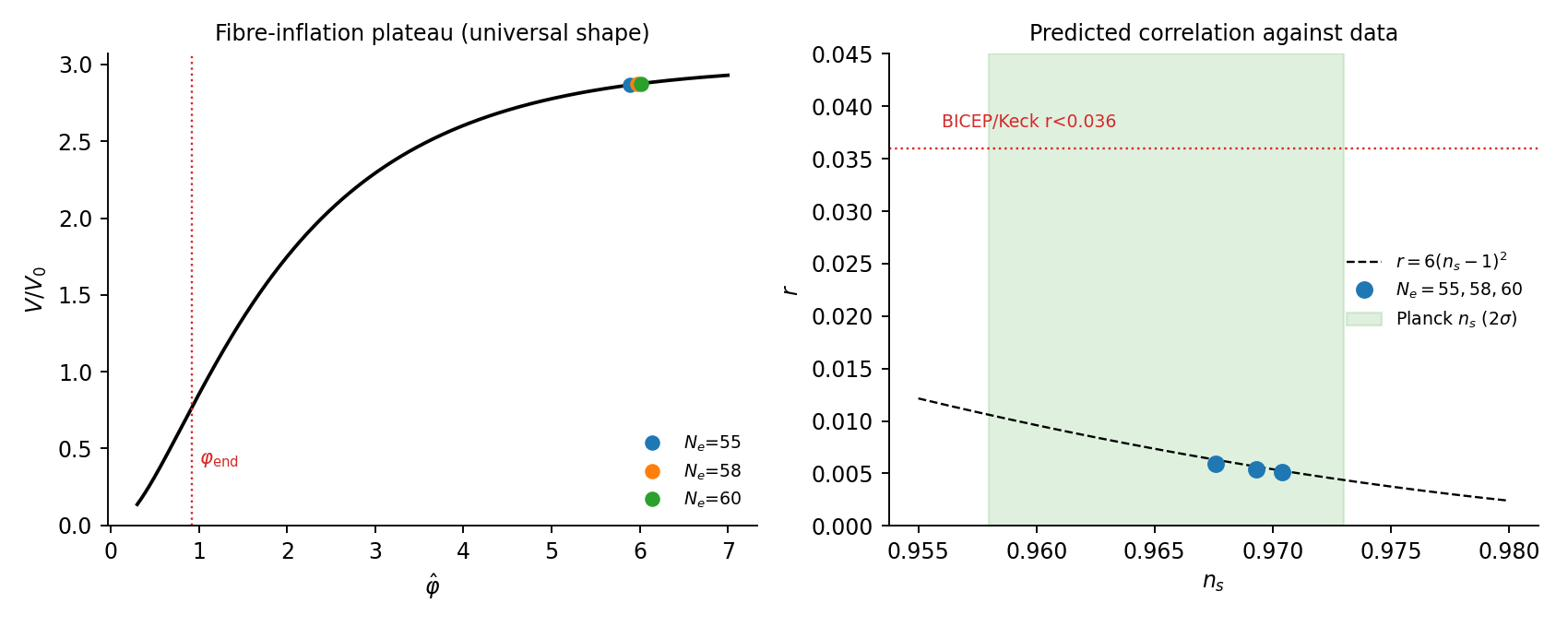
\includegraphics[width=.95\textwidth]{fig_inflation}
\caption{Left: the fibre-inflation plateau in the canonical field, with the horizon-exit points for $N_e=55,58,60$ and the end of inflation. Right: the predicted points on the $r$--$n_s$ plane against the correlation $r=6(n_s-1)^2$, the Planck $2\sigma$ band on $n_s$, and the BICEP/Keck bound on $r$.}\label{fig:inf}\end{figure}

\section{The amplitude fixes the scale, and why the geometry does not enter}
The COBE/Planck normalisation $A_s=V_0\,v(\varphi_*)/(24\pi^2\varepsilon_*)=2.1\times10^{-9}$, with $v(\varphi_*)\simeq2.87$ the plateau shape at horizon exit, gives
\begin{equation}
V_0\simeq5.9\times10^{-11}\,\MPl^4,\qquad M_{\rm inf}=V_0^{1/4}\simeq6.7\times10^{15}~\text{GeV}.
\end{equation}
\textbf{$V_0=24\pi^2\varepsilon_*A_s/v(\varphi_*)$ contains no intersection number, no volume and no loop coefficient.} Both $\varepsilon_*$ and $v$ are fixed by the plateau shape, universal for this class, and by $N_e$. \textbf{The chain $A_s\to V_0\to M_{\rm inf}$ is independent of which K3-fibred manifold is used}, which is why the reanchoring of \S6 leaves it untouched. What the loop coefficients do control is $R=16AC/B^2$, whose smallness ($\lesssim3\times10^{-5}$ for $N_e\gtrsim60$) bounds $C_W\gtrsim0.026$, comfortably inside the $O(0.1$--$1)$ range.

\paragraph{The sum rule and the inflation observables share a logic.} Both are protected from the loop coefficients, and by the same mechanism: the observable is a combination in which the unknown either cancels (the angle, in the sum rule) or enters only through a ratio that must be small anyway ($R$, in inflation). \textbf{The factor $2w_1=11$ between $c_b^2+c_b'^2=|\vec p|^2=0.2038$ and $\alpha_b^2+\alpha_b'^2=2.2414$ is essential and was omitted in an earlier draft.}

\section{Epistemic status}
\begin{center}\small
\begin{tabular}{lll}\toprule
quantity & status & note\\\midrule
sum rule, $2.2414$ & derived (exact) & machine precision\\
topological wall, $R_{\min}=8.34\,\mu$m & candidate & barrier exponent open\\
$\Lambda_4=\varepsilon^2(1/R)^4$ & candidate & tuning $10^{-2}$ declared\\
$\Omega_{\rm DM}/\Omega_b=6$ & candidate & one fitted O(1) factor\\
plateau shape, $\kappa=2/\sqrt3$, $r=6(n_s-1)^2$ & derived & standard fibre inflation\\
$n_s$, $r$ & predicted & fixed by $N_e$ alone\\
$A_s\to V_0\to M_{\rm inf}$ & fixed by normalisation & geometry-independent\\
divisor~1 even under the involution & \textbf{verified} & fixed by the involution\\
the two dP$_7$ exchanged by the involution & \textbf{open} & recompute Article~V statistics in the even basis\\\bottomrule
\end{tabular}
\end{center}
The last line deserves a sentence. Since the involution exchanges the two diagonal del Pezzo divisors, only their sum survives the projection, and the family statistics of Article~V --- which fixed both independently --- should be redone in the orientifold-even basis. The flat subspace remains two-dimensional, so the sum rule and its exactness are untouched; the individual projections would shift. \textit{[Open, declared.]}

\section{How this paper dies}
\emph{(i)} If a torsion balance finds Newton at $8.2\,\mu$m, the parent framework dies and both parts with it. \emph{(ii)} If $\Omega_{\rm DM}/\Omega_b$ is revised away from $5$--$6$, the projection reading fails. \emph{(iii)} If the substructure proves hierarchical and uncorrelated with any discrete angular structure, Layer~3 fails and Layers~1--2 survive. \emph{(iv)} If the barrier exponent moves $R_{\min}$ outside $8.2\pm0.5\,\mu$m, the topological wall fails. \emph{(v)} If the extrinsic-curvature identification requires $\varepsilon<10^{-3}$, the dark-energy claim is withdrawn. \emph{(vi)} If $n_s$ leaves $0.965$--$0.971$ or $r$ exceeds $0.01$, the fibre-inflation identification fails. \emph{(vii)} If $r=6(n_s-1)^2$ is violated, the plateau shape is wrong and Part~B collapses at its first step. \emph{(viii)} If the even-basis recomputation moves the family median of Article~V outside the window, the class statement of that article weakens --- the sum rule survives.


% ═══════════════════════════════════════════════════════════════════════════
%  APPENDICE DE LIAISON — identique dans les sept articles.
%  % ═══════════════════════════════════════════════════════════════════════════
%  APPENDICE DE LIAISON — identique dans les sept articles.
%  % ═══════════════════════════════════════════════════════════════════════════
%  APPENDICE DE LIAISON — identique dans les sept articles.
%  \input{appendix-where} juste avant \begin{thebibliography} ou la biblio.
%  Il répond à : qui vit où, et qu'est-ce que la série a changé en cours de route.
% ═══════════════════════════════════════════════════════════════════════════
\section*{Appendix: which sector lives where, and what changed}
\addcontentsline{toc}{section}{Appendix: which sector lives where}

The series was written over several months and \textbf{two of its assignments moved}.
A reader who meets the articles out of order is owed an explicit map rather than an
inference, so it is given here, identically in all seven papers.

\subsection*{A.1 The three locations}
The geometry has three places where physics can sit: the \emph{brane} at $y=0$,
the \emph{bulk} of the $8.2\,\mu$m interval, and the \emph{far wall} at $y=\pi R$.
\begin{center}\small
\begin{tabular}{llll}\toprule
sector & lives on & carried by & established in\\\midrule
ordinary matter & \textbf{brane} & thin core, Standard Model & I\\
gravity, radion, graviton & \textbf{bulk} & five-dimensional fields & I\\
the mediator $\Phi$ and its tower & \textbf{bulk} & Airy states of the $|y|$ well & II\\
the galactic response & \textbf{bulk} $\to$ brane & $\Phi$ exchange between baryons & III\\
dark matter & \textbf{see A.2} & --- & III, revisited in VI\\
dark energy & \textbf{see A.3} & --- & III, revisited in VI\\
hidden gauge sector & \textbf{far wall} & eight D8 and one O8 & V\\\bottomrule
\end{tabular}
\end{center}

\subsection*{A.2 Dark matter: the reservoir, and what the wall reading adds}
Articles~I--IV place dark matter in the \emph{bulk}: the excited states of the Airy
tower, populated cold at birth, collisionless, carrying at least $98.6\%$ of the dark
sector's density. That assignment does the work in three places. It makes structure
formation identical to cold dark matter at linear order. It answers the Bullet Cluster
by mass budget alone --- cluster masses are cluster masses, and the lensing tracks the
reservoir, which is why the lensing--dynamics difficulty of purely modified dynamics is
not inherited. And it fixes the radiation budget of Article~I.

Article~VI proposes a different reading: dark matter as the ordinary matter of the six
other regions of the same wall, seen through the bulk, giving
$\Omega_{\rm DM}/\Omega_b=N_{\rm regions}-1=6$ against an observed $5.31$.
\textbf{These are not the same statement, and we do not pretend otherwise.}

What they share is everything the phenomenology uses: in both readings the dark
component is cold, collisionless, and carries the mass, so lensing, the Bullet Cluster
and linear structure formation are unaffected. What differs is the \emph{constituent}:
quanta of $\Phi$ in the first, baryons of other regions in the second.
\textbf{The two are compatible if the tower reservoir is not required to be the whole
of the dark matter} --- and Article~III's own argument only requires it to dominate the
budget, not to be exhaustive. \Open

\subsection*{A.3 Dark energy: a bulk scalar, then a brane curvature}
Articles~I--IV treat $\Phi$ as the dark-energy candidate --- a bulk scalar engine. That
attempt \emph{failed by forty orders of magnitude}: a four-dimensional scalar cannot
reach $2.4$~meV from a $10^{-13}$~eV engine scale. The failure is recorded, not hidden.

Article~VI relocates dark energy \emph{to the brane}, as the extrinsic curvature of the
D8 wall in the cosmological bulk, $\Lambda_4=\varepsilon^2(1/R)^4$ with
$\varepsilon\simeq10^{-2}$. The mechanism supplies $(1/R)^4$ outright and leaves a gap
of $10^4$ rather than $10^{40}$. \textbf{$\Phi$ is correspondingly demoted from
dark-energy candidate to dark-sector mediator}, which is the role Articles~II and III
already gave it in every equation they actually use. \Candidate, declared tuning.

\subsection*{A.4 The radial acceleration relation, and what makes galaxies turn}
The relation is the one place where brane and bulk are \emph{both} indispensable, and
where nothing has moved since Article~III.

Baryons sit on the brane. They source $\Phi$, which propagates in the bulk with mass
$m_\Phi=24$~meV and hence Compton range $8.2\,\mu$m --- microscopic, so no fifth force
acts between laboratory bodies. What acts at galactic scale is not the free field but
the \emph{medium}: the coherent component of the dark sector responds to the baryonic
distribution, and that response, read back on the brane, is the extra acceleration.
The response saturates, which is why it produces a relation --- an acceleration scale
$g_\dagger$ --- rather than a rescaling of Newton's constant.

Three consequences, all in Article~III and unchanged:
\begin{itemize}\itemsep2pt
\item the response couples to the trace $T^\mu_{\ \mu}$, hence to mass and not to
      composition; the universality is bounded on 171 SPARC galaxies;
\item the response is carried by at most $1.4\%$ of the dark sector, the coherent part,
      so it never competes with the reservoir in the mass budget --- \textbf{galaxies
      turn because of the medium, they weigh because of the reservoir};
\item the response \emph{dies} in weak field, which is the ultra-diffuse galaxy test,
      and it dies in a decoherence bubble around the Sun, which is why Cassini is
      satisfied identically rather than by tuning.
\end{itemize}
\textbf{Neither relocation of A.2 or A.3 touches this.} The galactic response was never
assigned to the dark-energy sector, and it is not the reservoir either; it is the third
role, and it is the one the framework was built to explain.

\subsection*{A.5 What a reader should carry between articles}
Articles~I--IV stand on their own evidence and are not modified by V--VII: no result of
theirs is derived from the string embedding, and the embedding cannot promote any of
their labels. What V--VII add is an ultraviolet origin for one constant, a candidate
geometry, and two consequences of that geometry. What they \emph{change} is recorded
above and nowhere else: two relocations, both declared, neither retroactive.
 juste avant \begin{thebibliography} ou la biblio.
%  Il répond à : qui vit où, et qu'est-ce que la série a changé en cours de route.
% ═══════════════════════════════════════════════════════════════════════════
\section*{Appendix: which sector lives where, and what changed}
\addcontentsline{toc}{section}{Appendix: which sector lives where}

The series was written over several months and \textbf{two of its assignments moved}.
A reader who meets the articles out of order is owed an explicit map rather than an
inference, so it is given here, identically in all seven papers.

\subsection*{A.1 The three locations}
The geometry has three places where physics can sit: the \emph{brane} at $y=0$,
the \emph{bulk} of the $8.2\,\mu$m interval, and the \emph{far wall} at $y=\pi R$.
\begin{center}\small
\begin{tabular}{llll}\toprule
sector & lives on & carried by & established in\\\midrule
ordinary matter & \textbf{brane} & thin core, Standard Model & I\\
gravity, radion, graviton & \textbf{bulk} & five-dimensional fields & I\\
the mediator $\Phi$ and its tower & \textbf{bulk} & Airy states of the $|y|$ well & II\\
the galactic response & \textbf{bulk} $\to$ brane & $\Phi$ exchange between baryons & III\\
dark matter & \textbf{see A.2} & --- & III, revisited in VI\\
dark energy & \textbf{see A.3} & --- & III, revisited in VI\\
hidden gauge sector & \textbf{far wall} & eight D8 and one O8 & V\\\bottomrule
\end{tabular}
\end{center}

\subsection*{A.2 Dark matter: the reservoir, and what the wall reading adds}
Articles~I--IV place dark matter in the \emph{bulk}: the excited states of the Airy
tower, populated cold at birth, collisionless, carrying at least $98.6\%$ of the dark
sector's density. That assignment does the work in three places. It makes structure
formation identical to cold dark matter at linear order. It answers the Bullet Cluster
by mass budget alone --- cluster masses are cluster masses, and the lensing tracks the
reservoir, which is why the lensing--dynamics difficulty of purely modified dynamics is
not inherited. And it fixes the radiation budget of Article~I.

Article~VI proposes a different reading: dark matter as the ordinary matter of the six
other regions of the same wall, seen through the bulk, giving
$\Omega_{\rm DM}/\Omega_b=N_{\rm regions}-1=6$ against an observed $5.31$.
\textbf{These are not the same statement, and we do not pretend otherwise.}

What they share is everything the phenomenology uses: in both readings the dark
component is cold, collisionless, and carries the mass, so lensing, the Bullet Cluster
and linear structure formation are unaffected. What differs is the \emph{constituent}:
quanta of $\Phi$ in the first, baryons of other regions in the second.
\textbf{The two are compatible if the tower reservoir is not required to be the whole
of the dark matter} --- and Article~III's own argument only requires it to dominate the
budget, not to be exhaustive. \Open

\subsection*{A.3 Dark energy: a bulk scalar, then a brane curvature}
Articles~I--IV treat $\Phi$ as the dark-energy candidate --- a bulk scalar engine. That
attempt \emph{failed by forty orders of magnitude}: a four-dimensional scalar cannot
reach $2.4$~meV from a $10^{-13}$~eV engine scale. The failure is recorded, not hidden.

Article~VI relocates dark energy \emph{to the brane}, as the extrinsic curvature of the
D8 wall in the cosmological bulk, $\Lambda_4=\varepsilon^2(1/R)^4$ with
$\varepsilon\simeq10^{-2}$. The mechanism supplies $(1/R)^4$ outright and leaves a gap
of $10^4$ rather than $10^{40}$. \textbf{$\Phi$ is correspondingly demoted from
dark-energy candidate to dark-sector mediator}, which is the role Articles~II and III
already gave it in every equation they actually use. \Candidate, declared tuning.

\subsection*{A.4 The radial acceleration relation, and what makes galaxies turn}
The relation is the one place where brane and bulk are \emph{both} indispensable, and
where nothing has moved since Article~III.

Baryons sit on the brane. They source $\Phi$, which propagates in the bulk with mass
$m_\Phi=24$~meV and hence Compton range $8.2\,\mu$m --- microscopic, so no fifth force
acts between laboratory bodies. What acts at galactic scale is not the free field but
the \emph{medium}: the coherent component of the dark sector responds to the baryonic
distribution, and that response, read back on the brane, is the extra acceleration.
The response saturates, which is why it produces a relation --- an acceleration scale
$g_\dagger$ --- rather than a rescaling of Newton's constant.

Three consequences, all in Article~III and unchanged:
\begin{itemize}\itemsep2pt
\item the response couples to the trace $T^\mu_{\ \mu}$, hence to mass and not to
      composition; the universality is bounded on 171 SPARC galaxies;
\item the response is carried by at most $1.4\%$ of the dark sector, the coherent part,
      so it never competes with the reservoir in the mass budget --- \textbf{galaxies
      turn because of the medium, they weigh because of the reservoir};
\item the response \emph{dies} in weak field, which is the ultra-diffuse galaxy test,
      and it dies in a decoherence bubble around the Sun, which is why Cassini is
      satisfied identically rather than by tuning.
\end{itemize}
\textbf{Neither relocation of A.2 or A.3 touches this.} The galactic response was never
assigned to the dark-energy sector, and it is not the reservoir either; it is the third
role, and it is the one the framework was built to explain.

\subsection*{A.5 What a reader should carry between articles}
Articles~I--IV stand on their own evidence and are not modified by V--VII: no result of
theirs is derived from the string embedding, and the embedding cannot promote any of
their labels. What V--VII add is an ultraviolet origin for one constant, a candidate
geometry, and two consequences of that geometry. What they \emph{change} is recorded
above and nowhere else: two relocations, both declared, neither retroactive.
 juste avant \begin{thebibliography} ou la biblio.
%  Il répond à : qui vit où, et qu'est-ce que la série a changé en cours de route.
% ═══════════════════════════════════════════════════════════════════════════
\section*{Appendix: which sector lives where, and what changed}
\addcontentsline{toc}{section}{Appendix: which sector lives where}

The series was written over several months and \textbf{two of its assignments moved}.
A reader who meets the articles out of order is owed an explicit map rather than an
inference, so it is given here, identically in all seven papers.

\subsection*{A.1 The three locations}
The geometry has three places where physics can sit: the \emph{brane} at $y=0$,
the \emph{bulk} of the $8.2\,\mu$m interval, and the \emph{far wall} at $y=\pi R$.
\begin{center}\small
\begin{tabular}{llll}\toprule
sector & lives on & carried by & established in\\\midrule
ordinary matter & \textbf{brane} & thin core, Standard Model & I\\
gravity, radion, graviton & \textbf{bulk} & five-dimensional fields & I\\
the mediator $\Phi$ and its tower & \textbf{bulk} & Airy states of the $|y|$ well & II\\
the galactic response & \textbf{bulk} $\to$ brane & $\Phi$ exchange between baryons & III\\
dark matter & \textbf{see A.2} & --- & III, revisited in VI\\
dark energy & \textbf{see A.3} & --- & III, revisited in VI\\
hidden gauge sector & \textbf{far wall} & eight D8 and one O8 & V\\\bottomrule
\end{tabular}
\end{center}

\subsection*{A.2 Dark matter: the reservoir, and what the wall reading adds}
Articles~I--IV place dark matter in the \emph{bulk}: the excited states of the Airy
tower, populated cold at birth, collisionless, carrying at least $98.6\%$ of the dark
sector's density. That assignment does the work in three places. It makes structure
formation identical to cold dark matter at linear order. It answers the Bullet Cluster
by mass budget alone --- cluster masses are cluster masses, and the lensing tracks the
reservoir, which is why the lensing--dynamics difficulty of purely modified dynamics is
not inherited. And it fixes the radiation budget of Article~I.

Article~VI proposes a different reading: dark matter as the ordinary matter of the six
other regions of the same wall, seen through the bulk, giving
$\Omega_{\rm DM}/\Omega_b=N_{\rm regions}-1=6$ against an observed $5.31$.
\textbf{These are not the same statement, and we do not pretend otherwise.}

What they share is everything the phenomenology uses: in both readings the dark
component is cold, collisionless, and carries the mass, so lensing, the Bullet Cluster
and linear structure formation are unaffected. What differs is the \emph{constituent}:
quanta of $\Phi$ in the first, baryons of other regions in the second.
\textbf{The two are compatible if the tower reservoir is not required to be the whole
of the dark matter} --- and Article~III's own argument only requires it to dominate the
budget, not to be exhaustive. \Open

\subsection*{A.3 Dark energy: a bulk scalar, then a brane curvature}
Articles~I--IV treat $\Phi$ as the dark-energy candidate --- a bulk scalar engine. That
attempt \emph{failed by forty orders of magnitude}: a four-dimensional scalar cannot
reach $2.4$~meV from a $10^{-13}$~eV engine scale. The failure is recorded, not hidden.

Article~VI relocates dark energy \emph{to the brane}, as the extrinsic curvature of the
D8 wall in the cosmological bulk, $\Lambda_4=\varepsilon^2(1/R)^4$ with
$\varepsilon\simeq10^{-2}$. The mechanism supplies $(1/R)^4$ outright and leaves a gap
of $10^4$ rather than $10^{40}$. \textbf{$\Phi$ is correspondingly demoted from
dark-energy candidate to dark-sector mediator}, which is the role Articles~II and III
already gave it in every equation they actually use. \Candidate, declared tuning.

\subsection*{A.4 The radial acceleration relation, and what makes galaxies turn}
The relation is the one place where brane and bulk are \emph{both} indispensable, and
where nothing has moved since Article~III.

Baryons sit on the brane. They source $\Phi$, which propagates in the bulk with mass
$m_\Phi=24$~meV and hence Compton range $8.2\,\mu$m --- microscopic, so no fifth force
acts between laboratory bodies. What acts at galactic scale is not the free field but
the \emph{medium}: the coherent component of the dark sector responds to the baryonic
distribution, and that response, read back on the brane, is the extra acceleration.
The response saturates, which is why it produces a relation --- an acceleration scale
$g_\dagger$ --- rather than a rescaling of Newton's constant.

Three consequences, all in Article~III and unchanged:
\begin{itemize}\itemsep2pt
\item the response couples to the trace $T^\mu_{\ \mu}$, hence to mass and not to
      composition; the universality is bounded on 171 SPARC galaxies;
\item the response is carried by at most $1.4\%$ of the dark sector, the coherent part,
      so it never competes with the reservoir in the mass budget --- \textbf{galaxies
      turn because of the medium, they weigh because of the reservoir};
\item the response \emph{dies} in weak field, which is the ultra-diffuse galaxy test,
      and it dies in a decoherence bubble around the Sun, which is why Cassini is
      satisfied identically rather than by tuning.
\end{itemize}
\textbf{Neither relocation of A.2 or A.3 touches this.} The galactic response was never
assigned to the dark-energy sector, and it is not the reservoir either; it is the third
role, and it is the one the framework was built to explain.

\subsection*{A.5 What a reader should carry between articles}
Articles~I--IV stand on their own evidence and are not modified by V--VII: no result of
theirs is derived from the string embedding, and the embedding cannot promote any of
their labels. What V--VII add is an ultraviolet origin for one constant, a candidate
geometry, and two consequences of that geometry. What they \emph{change} is recorded
above and nowhere else: two relocations, both declared, neither retroactive.

\toolsstatement
\traceability{6}{The sum rule, the topological wall, the dark-energy scales and the inflation observables are produced by \texttt{scripts/verify.py}; the four figures by \texttt{scripts/figures.py}.}
\bibliographystyle{unsrt}\bibliography{ddf-refs}
\end{document}
